\documentclass{llncs}
\usepackage{llncsdoc}
\usepackage{epsfig}

%
\begin{document}
\def\addtocontents#1#2{}%
\def\addcontentsline#1#2#3{}%
\def\markboth#1#2{}%
%
\title{Towards Reconfigurable High Performance Computing for scientific many-body simulations}

\author{Tsuyoshi Hamada\inst{1}, Naohito Nakasato\inst{1}}

\institute{Computational Astrophysics Group,\\
The Physical and Chemical Research Institute (RIKEN),\\
Wako, Saitama 351-0198, Japan}

\maketitle
%
\begin{abstract}
This paper describes a methodology for implementing FPGA-based
accelerator from a high-level specification in a small special-purpose
language.  The idea is to generate, from a high-level description, (a)
a suitable configuration file for the FPGAs, (b) the C source code for
interfacing with the FPGA-based processors that has been generated,
and (c) a software emulator. The FPGA configuration is build by
combining components from a library of parametrized arithmetic
modules; these modules implement fixed point, floating point and
logarithmic numbers with flexible bitwidth and pipeline stages.  To
prove our methodology to be correct, we developed PROGRAPE-3 system as
a target hardware platform and implemented $N$-body calculation
algorithm using PGR.  With the PROGRAPE-3 system of a minimum
composition, we have achieved peak performance of 162 Gflops and
mesured performance of 100 Gflops on actual numerical simulation.
In the FPGA-based high performance computing area,
our methodology and implementation is wonderful for all to exist in world.
\end{abstract}
%
\section{Introduction}
%
In scientific simulations, there are much demand for high performance computer.
A lot of effort has been dedicated to super computing or high
performance computing(HPC) architecture in scientific computations.
Almost of these efforts are concentrated to general-purpose
processors(GPPs) or digital signal processors(DSPs), which have an
instruction-set architecture.  These have evolved receiving the
improvement of the integrated circuit technology.  Currently making
circuit to smaller begins to end, the situation has become doubtful.

The methodology of special-purpose computer receives much attention in
scientific simulation. In the astrophysical many-body simulation,
GRAPE(GRAvity piPE) system is useful 


In the scientific many-body simulations, an earlier example
of the develepment of reconfigurable hardware is
PROGRAPE-1(PROgrammable GRAPE-1)\ref{Hamada2000}.  PROGRAPE-1 is an
FPGA-based accelerator for many-body simulations.  It is implemented
with two Altera EPF10K100 FPGAs, each of which contains about 100k
gates.  The peak performance of calculating gravitational force
results in 0.96 Gflops.

Another earlier example similar to PROGRAPE-1 is RACE-1 which is
also develeped to accelerate Smoothed Particle Hydrodynamics(SPH)
simulation used in astrophysics. RACE-1 contains one Virtex XC2V3000 FPGA,
each of which contains about 3M gates. The peak performance of calculating 
Currently a part of the calculation seems to have been mounted now, and to become 3.6
Gflops.


Some peoples are tring to cut a novel HPC paradigm open with the
reconfigurable computing. 


Another
developed efficient floating-point library or modules generator,
design language or compiler. These are fragments of total solution for
applying the reconfigurable system to HPC.




But PROGRAPE-1 was necessary to do the programming by using HDL so this machine was not so handled.

programming was 

.  PROGRAPE-1
was composed of short length(14-bit) logarithmic arithmetics and this
was the reason why the performance was excelent with this outdated
FPGAs.

After pioneering development of Splash-1/2 \cite{Splash},
a number of FPGA-based reconfigurable system/accelarator (hereafter FBA)
such as PRISM \cite{W93}, PeRLe-0/1 \cite{VBRSTB94}
are proposed, developed and widely used in several research area.
Especially, it has been shown that an FBA is very effective for
problems which only need bit-operation or integer-operations
such as pattern matching, or image recognition, etc.
To be more specific, a pattern matching between two strings
can be easily implemented by the dynamic programming algorithm \cite{DP}
as a logic on FPGAs \cite{Splash}.
Their system have achieved 280 times better performance than
a supercomputer system (CM-2 with 64k nodes) at that time.

\begin{figure}[htb]
\begin{center}
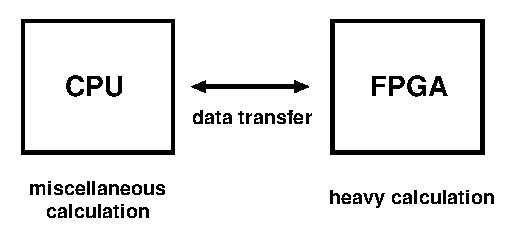
\includegraphics[angle=+0,width=8cm]{./mat/CPU-BOARD.eps}
\caption{Co-processor type Reconfigurable System.}
\label{CPU-BOARD}
\end{center}
\end{figure}

There are two types of an FBA; standalone type and co-processor type.
In the case of standalone type system, all arithmetic/computational operations
are implemented as logics on FPGAs and working by itself.
On the other hand, co-processor type system behaves as an add-in processor 
to a conventional computer (host computer).
In most cases, a host computer and a co-processor type system 
are connected by an external bus, e.g., PCI, PCI-X, or PCI-Express etc., 
and the host and the FBA work cooperationally (Figure \ref{CPU-BOARD}).
In this case, only a part of a problem
that should be a most computationally dominant part of the problem
is implemented as logics on FPGAs and
a remaining part of the problem is processed by the host computer.
For example, in astrophysical many-body simulations, 
we integrate equations of motion for gravitationally interacting particles,
and a most computationally dominant part of the problem is 
computation of gravitational interaction that has O($N^2$) dependency
on a number of particles $N$.
The computation of gravity is a part that should be implemented on 
an FBA and other part (e.g., integration of equations of motion)
is computed by the host computer.
In this paper, we present our results of considerable efforts
to make use of an FBA easy.
Especially, we have made a special attention to numerical simulations, 
such as the many-body problem as explained above, on an FBA.
We are now developing a software package named as
Processors Generator for Reconfigurable system (PGR package)

There are three motivations which let us to start the development of
PGR; First, there is little software support for 
using an FBA for computationally intensive
numerical problem, e.g., astrophysical simulations in our case.
In the astrophysics community, the success of the
GRAPE project \cite{GRAPE} shows us a great possibility of 
developing special purpose hardware system to accelerate 
numerical simulations. In the recent GRAPE project, specially
developed LSIs, which are mounted on a expansion board
for a host computer, are used as a computing engine.
However, total development costs of most recent generation of the
GRAPE system already reaches 5 million \$ and most of the cost
was devoted to initial development of LSIs. 
Such big budget become a barrier for constructing a new generation system
or new LSI for other kind of astrophysical simulations.
Now, using FPGAs as a computing engine 
to accelerate numerical simulations is becoming 
feasible and a practical alternative to ASICs 
as shown in \cite{Hamada2000}.
They have shown a possibility of an FBA (PROGRAPE-1 system)
as the computing engine for astrophysical simulations.
In their work, primitive operations such as addition, subtraction, 
and multiplication etc., numerical algorithm itself, I/O, and control logic
have been implemented by VHDL from full-scratch
since there was a no software support for implementing
numerical calculations on FPGAs at that time.
Especially, there was (and still now is)
no suitable floating-point operations IP core for their and our purpose.
As shown in \cite{Makino1990}, surprisingly small number of digits
(say mantissa 3 bits) is sufficient for a kind of astrophysical many-body problem.
However, available IP cores of floating-point operations
from a several vendors are not efficient for our purpose of reduced accuracy.
This is the first reason and the strong motivation to develop 
parametrized arithmetic modules with support of 
arbitrary bit-length floating-point operations, 
which is a core and base of the PGR package.

\begin{table*}
\caption{Comparisons of co-processor type reconfigurable system}
\begin{center}
\begin{tabular}{lcccc}
\hline
\hline
& Cray XD1 & SGI Altix & SRC  & PROGRAPE-3 \\
\hline
host CPU                & Opteron  & Itanium   & Xeon & Pentium4/Opteron \\
bandwidth (GB s$^{-1}$) & 3.2      & TBD       & 2.6  & 0.5              \\
A number of FGPAs       & 6        & TBD       & unknown & 4             \\
\hline
\hline
\end{tabular}
\end{center}
\label{comparison}
\end{table*}

Secondly, a few recently released computing system such as Cray XD1 
has FPGAs as co-processors and this is exactly a co-processor type FBA.
Although we have already developed a largest FBA (PROGPRAE-3 board)
with 4 Xilinx XC2VP70 chips for our purpose, 
an advantage of such system developed by high performance computing vendors
over the PROGRAPE-3 is high speed bandwidth between the host computer (CPU)
and FPGAs. Table \ref{comparison} shows comparisons between our board
and available/planed HPC system with FPGAs by three vendors.
High bandwidth will certainly expands area of applications because ratio between 
number of floating-point operations and input data size (in a number of operations per byte)
strongly depends on a kind of applications. 
An example of an application that has a large number of operations per byte
is matrix multiplication (O($N$) dependence on a number of element),
and an application that has opposite nature is discrete fourier transform (O($N^2$) dependence).
Note astrophysical gravitational many-body simulations also do not need high bandwidth
and this is a reason why the GRAPE project has been greatly succeeded 
with even modest bandwidth of $\sim$ 0.13 GB s$^{-1}$.
This possibility strongly encourage us to develop the PGR package
that supports not only our PROGRAPE-3 but an general FBA such as Cray XD1.

\begin{figure*}[htb]
\begin{center}
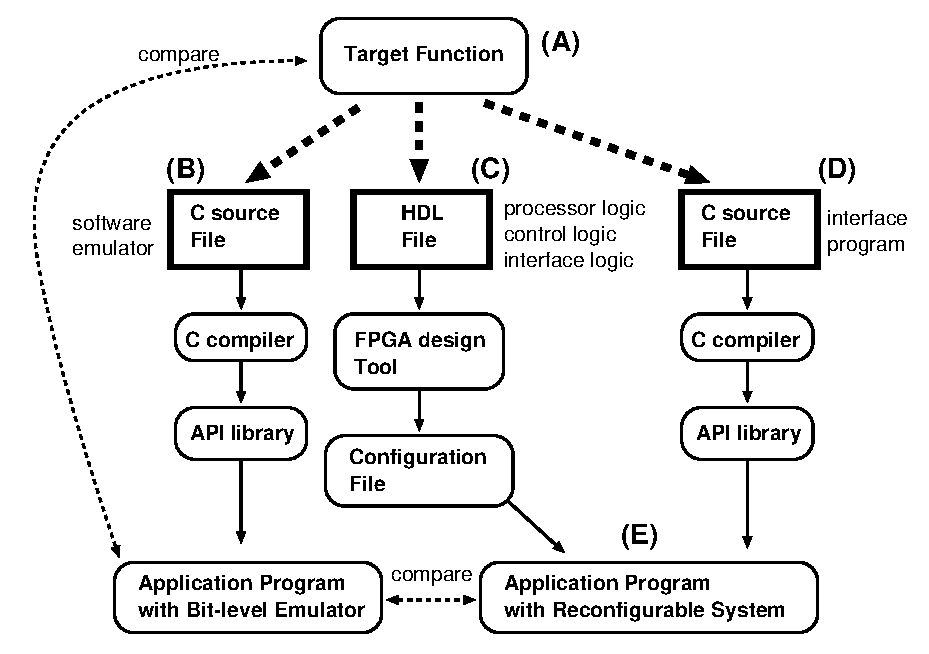
\includegraphics[angle=+0,width=12cm]{./mat/tradflow.eps}
\caption{Conventional work flow for implementing an application on a RS system.}
\label{tradflow}
\end{center}
\end{figure*}

A third motivation is that even if implementing a simplest
application on FPGAs is very difficult and tough work for
possible users in many fields that demand strong computational resources.
This is because conventional work flow for designing and implementing
an FBA is much more complicated than 
conventional programming in C or Fortran languages.
Figure \ref{tradflow} shows conventional work flow for
implementing an application on an FBA.
The work flow consists of the following five steps.

\begin{itemize}
\setlength{\itemsep}{6pt}

\item[(A)] Target Function Specification:
We specify a target function, namely the function that pipeline
processors calculate. This step includes to specify 
data flow for the calculation of the target function, 
and input and output number format and word length for each arithmetic operation. 

\item[(B)] Bit-Level Software Emulator:
We develop a software emulator which implements the target function
defined in step (A). Using this software emulator, we verify
whether the designed hardware can actually calculate the target
function with required accuracy. In this step, we also define the
application program interface (API). 

\item[(C)]  Hardware Design:
In this step, we actually write the source code which implements the
pipeline processors in a hardware description language (HDL) such as VHDL.
In addition, we design the control logic and host interface logic also
in some HDL. The HDL description is compiled to the configuration data
for the FPGAs by a CAD software, usually provided by the
manufacturer of the FPGA device.

\item[(D)] Interface Software:
We develop the software on the host computer which takes care of the
communication to the FBA and data format conversion between the
floating-point data on the host and specialized data format used on
the developed pipeline processors. The developed software should have
the same API as that of the software emulator developed in step (B).

\item[(E)] Finally, we can actually use the FBA with
real application program.
\end{itemize}

In these steps, we have to design, test, and debug a large amount of hardware logics
and softwares. Of course, many of the softwares and hardware designs can
be reused, when we develop different applications. For example, the
design of the floating-point multiplier is rather generic, and can be
used in almost any application. Also, it is possible to buy 
IP cores of such designs.
However, just to understand how to use the IP cores, one need a deep understanding
of details of the IP cores. Thus, even
though the reusability significantly reduce the amount of the work
needed for the second and later design for a person, the initial
hurdle remains rather high, for a person who has never used 
such IP core, or actually the availability of the IP cores make the hurdle
even higher, since a starter needs to understand, in addition to the
basics of the hardware design and HDL, the use of such IP cores.
Furthermore, a price of IP cores is quite expensive in general for a academic 
researcher and it is not always true that there are suitable IP cores
for one's purpose as explained above.

The development of a communication software is generally even more
difficult than the design of the hardware, since it requires the
knowledge of how a device driver work in the operating
system of the host computer, and infinite number of small details;
how to integrate the device driver to the operating system, how to
correctly generate the compiler flags to compile the device driver and so on.
All these works combined make it almost impossible 
for possible users to even think of implementing the pipeline processor on an FBA.

In theory, most of the softwares and hardware descriptions,
including the bit-level design of the pipeline processors itself,
can be automatically generated from some high-level description of the
pipeline. The basic idea behind the PGR package,
which we will describe details in this paper,
is to provide such automatic generation.
The PGR package analyzes a description of pipeline processors
written in the PGR Description Language (PGDL) as input
and then translates and generates necessary hardware descriptions, 
a bit-level emulator, and communication softwares.
Namely, a possible user of an FBA can concentrate on writing their
application in the PGDL.
This means that the PGR system can drastically reduce the amount of
the work (and needed knowledge) of such user.
More importantly, the PGDL does not depends on a specific hardware
(e.g., PROGRAPE-3) and this make it possible to
reuse a application written in the PGDL on a newly developed FBA
when the PGR package supports the new FBA.
The effort spent to design one application on
one hardware will not be thrown away when a new hardware becomes available.

In this paper, we describe details of the PGR package
that makes a design flow of an FBA much simpler than
the conventional design flow.
In section 2, we present a basic idea behind the PGR package
and describe details of our newly developed parametrized 
floating-point arithmetic modules that are key components of the PGR package.
Moreover, we show a simple design example using the PGDL.
In section 3, we describe an example of a real application 
and show obtained performance on the PROGRAPE-3.
Finally, we summarize our results in section 4.
%
\section{PGR : Processors Generator for Reconfigurable systems}
\subsection{Basic idea behind the PGR system}

If we inspect Figure \ref{tradflow} again, we can see the fact that
{\bfseries all} softwares and hardware description is derived from the
target function specification in step (A). Thus, it should be possible
for a sufficiently smart software to generate all necessary softwares
and hardware descriptions from the target function description written
in some high-level language. The basic idea of PGR is to develop such
a smart software.

\begin{figure*}[htb]
\begin{center}
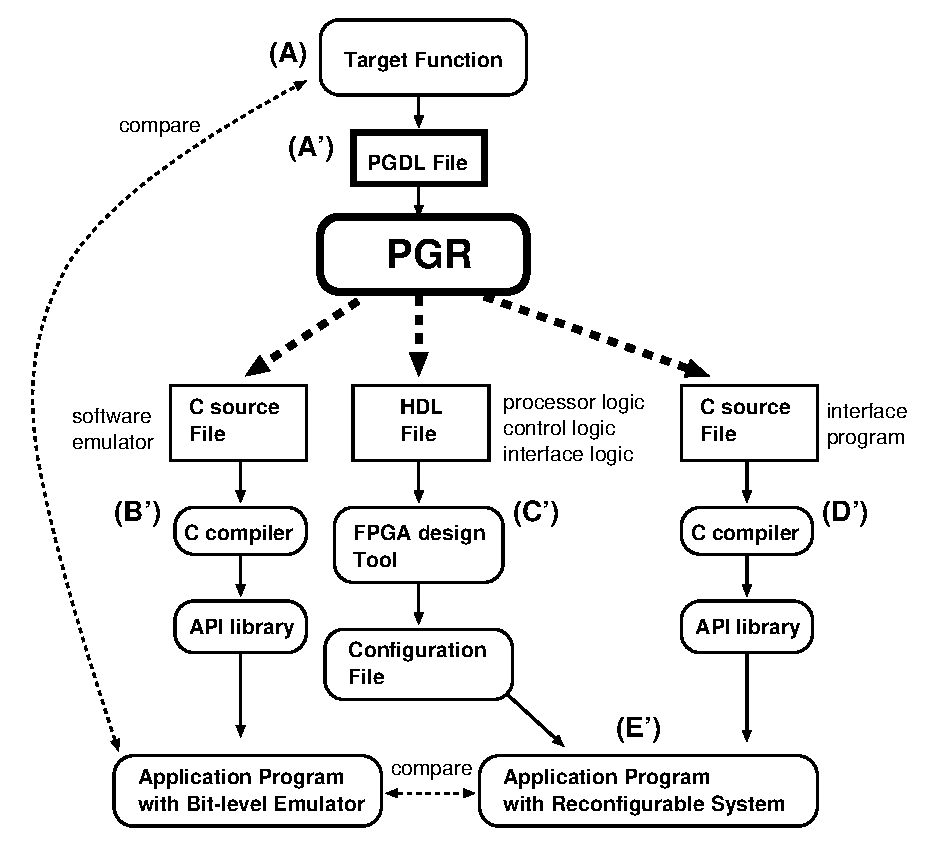
\includegraphics[angle=+0,width=12cm]{./mat/pgrflow.eps}
\caption{How the design flow changes with PGR.}
\label{pgrflow}
\end{center}
\end{figure*}

Figure \ref{pgrflow} shows how the design flow changes with the PGR package.
After we define a target function, then we write it in the PGDL
(see the later section for details on the PGDL).
The PGR software system takes this PGDL description of the pipeline processors
as input, and generates all softwares and hardware descriptions.
Thus, with the PGR package, a user do not have to write HDL source codes for
the processor and C source codes for a communication software.

\subsection{PGR five layers model}
To make the PGR software system independent on a specific hardware,
we create the PGR five layers model which divide 
an FBA into five parts.
Figure \ref{fig5model} shows the PGR five layers model, 
and it's composed of User Program Layer(UPL), API Layer(APL),
Device Driver Layer(DDL), I/O \& Control Logic Layer(ICL) and
Arithmetic Logic Layer(ALL).

The UPL is a user application which communicates
with an FBA through the APL.
The APL contains the top level API implementations that
doesn't depend on an individual FBA.
The DDL consists of both a low level communication library and a device driver software. 
The ICL is a glue logic such as the PCI interface logic and 
local I/O logic on an FBA.
The ALL is composed of parametrized arithmetic modules,
details of which is described later, 
and control logic of pipeline processors.

The PGR package generates only the layers that doesn't depend on 
a specific FBA, namely the APL and ALL.
The others layers (DDL and ICL) depend on hardware specification
of the FBA such as architecture of a host computer, used operating
system, or a type of inter-connection hardware (e.g., PCI, PCI-Express and so on).
We define standard specifications between the hardware depended layers(DDL,ICL)
and the independent layers(APL,ALL).
Our current target hardware is the PROGRAPE-3 board (see figure\ref{figpg3}).
The inter-connection hardware of the PROGRAPE-3 is the 66 MHz, 64 bit PCI bus
and detailed implementation of the ICL for PROGRAPE-3
is shown in Figure\ref{figicl}.

\begin{figure}[htb]
\begin{center}
  \begin{minipage}{.45\linewidth}
    \begin{center}
    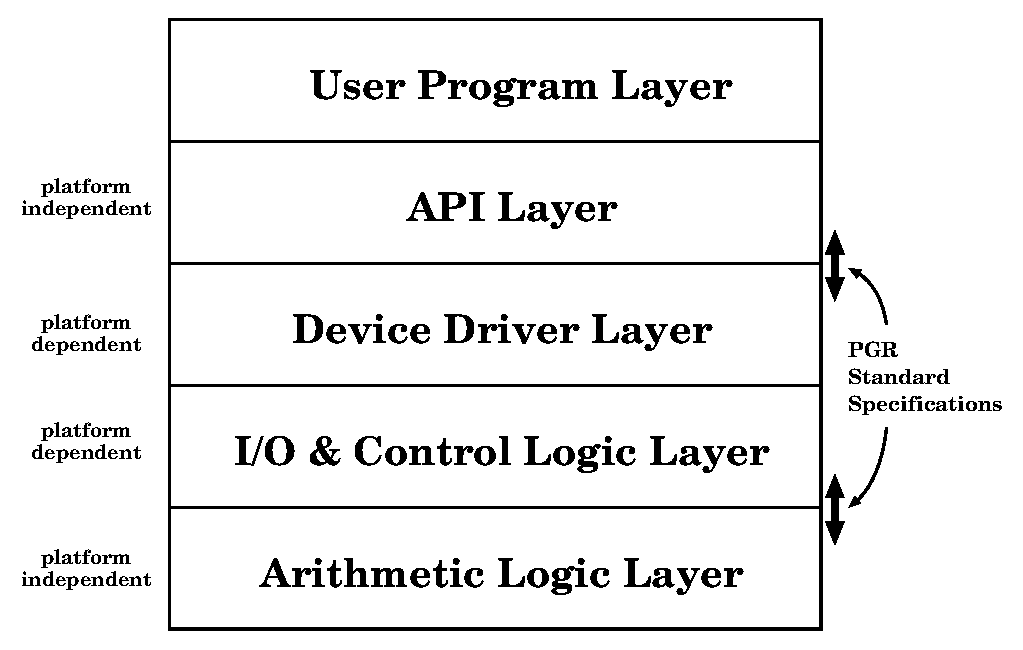
\includegraphics[angle=+0, width=1.2 \linewidth]{./mat/5model.eps}
    \caption{PGR five layers model.}
    \label{fig5model}
    \end{center}
  \end{minipage}
  \hspace{2.4pc}
  \begin{minipage}{.45\linewidth}
    \begin{center}
    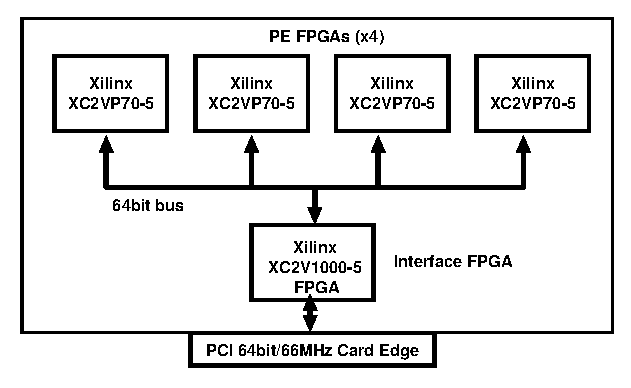
\includegraphics[angle=+0,width=1.2 \linewidth]{./mat/pg3.eps}
    \caption{PROGRAPE-3 board structure}
    \end{center}
  \end{minipage}
\end{center}
\end{figure}



\begin{figure}[htb]
\begin{center}
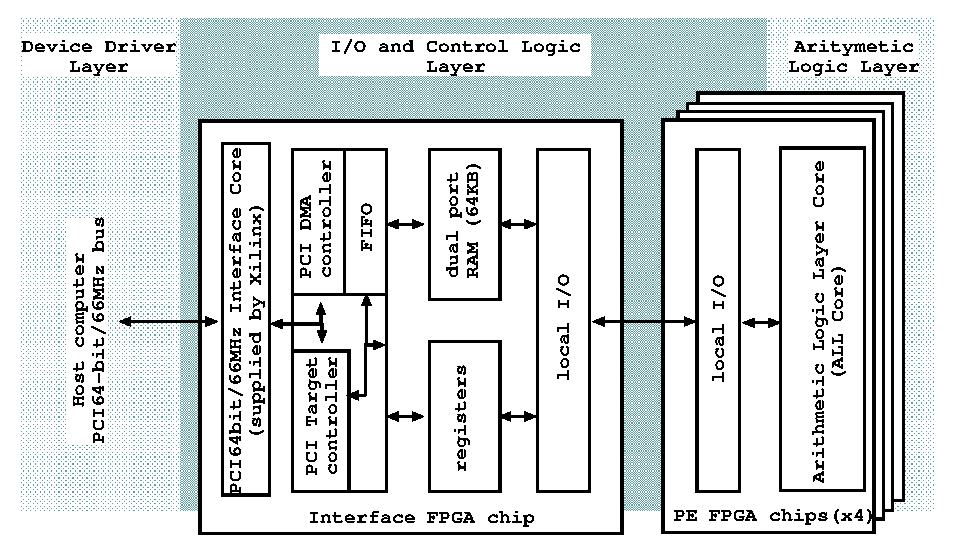
\includegraphics[angle=+0,width=8cm]{./mat/pgr_icl.eps}
\caption{real implementation of ICL.}
\label{figicl}
\end{center}
\end{figure}

\subsection{Parametrized Arithmetic Modules}
The parametrized arithmetic modules are the most low-level components
for the PGR package such as addition, subtraction, 
multiplication, division, and square-root, etc. 
Currently, the PGR package supports
29 parametrized arithmetic modules as shown in table \ref{tabpgmod}.

In this table, modules with {\tt pg\_float} are floating point format arithmetics.
We define internal floating-point format as 1-bit for a sign, 
1-bit for a non-zero expression, $n$-bit for exponent, 
and $m$-bit for mantissa, where $m$ and $n$ can be 
changed arbitrary up to single-precision for floating-point in the PGDL.
For example, in the PGDL, we can use float-point addition
as follows;
\begin{verbatim}
pg_float_add(x,y,z,26,16,1);
\end{verbatim}
Here, the arguments inside of parentheses indicate
the first input, the second input, output, total bit-length
of floating-point format, bit-length for mantissa,
and number of pipeline stages, respectively,
from the first to sixth argument.
This particular example expresses 
$z = x + y$, where $x,y,z$ are 26-bit floating numbers (mantissa is 16-bit).
And a number of pipeline stage for this arithmetic is one.
We note that for the rounding operation in the PGR package,
we have implemented nine types of several options that
also can be changed by a hidden argument in the PGDL.
If this argument is omitted like above example, 
a rounding to the nearest even is selected.

\begin{table}
\caption{PGDL Parametrized Arithmetic Modules}
\begin{center}
\begin{tabular}{ll}
\hline
\hline
Parametrized Arithmetic Module &  arithmetic\\
\hline
floating point format & \\
 {\tt pg\_float\_add}           &  $+$\\
 {\tt pg\_float\_unsigned\_add} &  $+$ (unsigned)\\
 {\tt pg\_float\_sub}           &  $-$\\
 {\tt pg\_float\_unsigned\_sub} &  $-$ (unsigned)\\
 {\tt pg\_float\_mult}          &  $\times$\\
 {\tt pg\_float\_div}           &  $/$ \\
 {\tt pg\_float\_sqrt}          &  $\sqrt{x}$ \\
 {\tt pg\_float\_square}        &  $x^2$\\
 {\tt pg\_float\_recipro}       &  $x^{-1}$\\
 {\tt pg\_float\_negate}        &  $\times -1.0$\\
 {\tt pg\_float\_compare}       &  compare\\
 {\tt pg\_float\_compare\_abs}  &  compare\\
 {\tt pg\_float\_compz}         &  compare to 0\\
 {\tt pg\_float\_compz\_abs}    &  compare to 0\\
 {\tt pg\_float\_accum}         &  accumulate\\
 {\tt pg\_float\_unsigned\_accum}&  accumulate (unsigned)\\
 {\tt pg\_float\_fixaccum}      &  accumulate\\
fixed point format & \\
 {\tt pg\_fix\_addsub}          &  $+$, $-$\\
 {\tt pg\_fix\_mult}            &  $\times$\\
 {\tt pg\_fix\_unsigned\_mult}  &  $\times$ (unsigned)\\
 {\tt pg\_fix\_accum}           &  accumulate\\
logarithmic format& \\
 {\tt pg\_log\_add}             &  $+$\\
 {\tt pg\_log\_unsigned\_add}   &  $+$ (unsigned)\\
 {\tt pg\_log\_muldiv}          &  $\times$, $/$\\
 {\tt pg\_log\_shift}           &  $\sqrt{x}$, $x^2$\\
format conversion & \\
 {\tt pg\_conv\_fixtofloat}     &  fix $\Rightarrow$ float\\
 {\tt pg\_conv\_floattofix}     &  float $\Rightarrow$ fix\\
 {\tt pg\_conv\_ftol}           &  fix $\Rightarrow$ log\\
 {\tt pg\_conv\_ltof}           &  log $\Rightarrow$ fix\\
\hline
\hline
\end{tabular}
\end{center}
\label{tabpgmod}
\end{table}

Modules {\tt pg\_fix\_addsub} and {\tt
pg\_fix\_accum} are fixed point format adder/subtracter and
accumulator, respectively.  Modules {\tt pg\_log\_muldiv} and {\tt
pg\_log\_unsigned\_add} are logarithmic format multiplier/divider and
unsigned adder, respectively. In the logarithmic format, a positive,
non-zero real number $x$ is represented by its base-2 logarithm $y$ as
$x=2^{y}$.
This logarithmic format is useful because 
it has larger dynamics length for the same word length and
operation such as multiplication and square root
are easier to implement than in the usual floating-point format.
As a result, the logarithmic format has been adapted for the
gravitational pipelines in low-accuracy type GRAPE-1,3,5 systems.
For more details of the logarithmic format, see GRAPE-5 paper
\cite{KFMT00}.
Module {\tt pg\_log\_shift} is a logarithmic format
shifter. Shift operations in the logarithmic format express square
(left shift) and squared root (right shift). 

Modules with {\tt pg\_conv} are converters from a particular format
into another format, e.g., {\tt pg\_conv\_floattofix} converts
a floating-point number into a corresponding fixed point number.

In tables \ref{tabpg_float_mult}, \ref{tabpg_float_unsigned_add},
\ref{tabpg_float_sqrt}, \ref{tabpg_float_recipro},
\ref{tabpg_log_unsigned_add}, and \ref{tabpg_fix_accum}, we illustrate
resource consumption and clock frequency of several important
parametrized arithmetic modules.
Despite we have implemented all of the parametrized arithmetic modules
from full scratch by ourself, 
the obtained performance results for each module
are almost same as other good implementations such as Manheim's (\cite{GKM02}).



\begin{table}
  \begin{center}
    \begin{minipage}{.45\linewidth}
      \caption{Multiplier(floating point)}
      \begin{center}
	\begin{tabular}{cccrr}
	  \hline
	  \hline
	  length  & length(mantissa) & stages & MHz & slices\\
	  \hline
	  18   &  9 & 2 & 290.192 &  31 \\
	  &    & 0 & 133.387 &  15 \\
	  \hline
	  26   & 17 & 4 & 224.266 &  56 \\
	  &    & 2 & 151.953 &  41 \\
	  &    & 0 &  80.762 &  23 \\
	  \hline
	  33   & 24 & 3 & 136.986 &  93 \\
	  &    & 0 &  68.847 &  56\\
	  \hline
	  \hline
	\end{tabular}
      \end{center}
      \label{tabpg_float_mult}
    \end{minipage}
    \hspace{2.4pc}
    \begin{minipage}{.45\linewidth}
      \caption{Multiplier(floating point)}
      \begin{center}
	\begin{tabular}{cccrr}
	  \hline
	  \hline
	  length  & length(mantissa) & stages & MHz & slices\\
	  \hline
	  18   &  9 & 2 & 290.192 &  31 \\
	  &    & 0 & 133.387 &  15 \\
	  \hline
	  26   & 17 & 4 & 224.266 &  56 \\
	  &    & 2 & 151.953 &  41 \\
	  &    & 0 &  80.762 &  23 \\
	  \hline
	  33   & 24 & 3 & 136.986 &  93 \\
	  &    & 0 &  68.847 &  56\\
	  \hline
	  \hline
	\end{tabular}
      \end{center}
      \label{tabpg_float_mult}
    \end{minipage}
  \end{center}

  \begin{center}
    \begin{minipage}{.45\linewidth}
      \caption{Square root (floating point)}
      \begin{center}
	\begin{tabular}{cccrr}
	  \hline
	  \hline
	  length  & length(mantissa) & stages & MHz & slices\\
	  \hline
	  18   &  9 & 4 & 215.517 & 86 \\
	  &    & 2 & 157.754 & 71 \\
	  &    & 0 &  79.971 & 51 \\
	  \hline
	  26   & 17 & 4 & 188.964 & 140 \\
	  &    & 2 & 127.959 & 116 \\
	  &    & 0 &  56.500 &  84 \\
	  \hline
	  33   & 24 & 5 & 141.243 & 425 \\
	  &    & 3 & 104.998 & 392 \\
	  &    & 1 &  70.210 & 374 \\
	  \hline
	  \hline
	\end{tabular}
      \end{center}
      \label{tabpg_float_sqrt}
    \end{minipage}
    \hspace{2.4pc}
    \begin{minipage}{.45\linewidth}
      \caption{Adder (logarithmic number)}
      \begin{center}
	\begin{tabular}{cccrr}
	  \hline
	  \hline
	  length  & length(mantissa) & stages & MHz & slices\\
	  \hline
	  14   &  6 & 4 & 201.077 & 94 \\
	  &    & 2 & 151.207 & 73 \\
	  &    & 0 &  64.545 & 57 \\
	  \hline
	  17   &  9 & 5 & 195.369 & 116 \\
	  &    & 2 & 138.042 &  92 \\
	  &    & 0 &  58.828 &  86 \\
	  \hline
	  20   & 12 & 6 & 218.293 & 191 \\
	  &    & 2 & 135.125 & 123 \\
	  &    & 0 &  53.562 & 115 \\
	  \hline
	  \hline
	\end{tabular}
      \end{center}
      \label{tabpg_log_unsigned_add}
    \end{minipage}
  \end{center}
\end{table}


\subsection{PGDL: PGR Description Language}
In this subsection, we illustrate how pipeline processors are
specified in the PGDL and how such description is translated
into the hardware description of pipelined processors.

\begin{figure}[htb]
\begin{center}
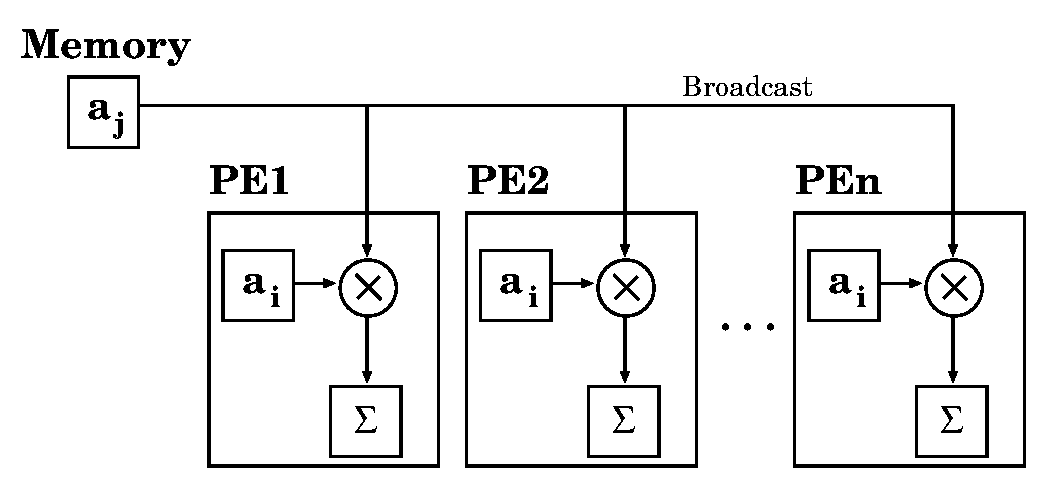
\includegraphics[angle=+0,width=8cm]{./mat/simple.eps}
\caption{Block diagram of the example processors(PEs).}
\label{fig4}
\end{center}
\end{figure}

With the current version of the PGR package, it is specially tuned
to generate hardware description of pipelined processors
for the following summation form;
\begin{equation}
f_i = \sum_{j = 1}^{n} F(\boldmath{p}_i, \boldmath{p}_j),
\end{equation}
where $f_i$ is summation for $i$-th data, $\boldmath{p}_i$ are
some values associated with $i$-th data, and
$F$ expresses calculations where $i$-th and $j$-th data are as inputs.

As an example target, we consider the following artificial calculations;
\begin{equation}
f_i = \sum_j^n {a_i a_j}.\qquad (i=1,...,n)
\end{equation}
Figure \ref{fig4} shows the block diagram
for this target processor.
Here, $a_i$ and $a_j$ are scalar values for $i$-th and
$j$-th elements, respectively.
This target simply calculates a product of $a_i$ and $a_j$, 
and sums the product up for all $j$.
In this example, we have the essential ingredients of an FBA:
data, their representation, functional form of arithmetic operations
between data $i$ and $j$.

Figure \ref{fig5} shows the PGDL description of this target function.
The first two lines define the bit-length of the floating-point format.
These definitions are actually used in the next block
(three lines starting with ``/''),
which defines the register and memory layout,
which also determine the interface API etc. 
For the data $a_i$ (and $a_j$), we use a floating point format,
with 26 bits in total (1-bit for sign, 1-bit for non-zero flag, 8-bits
for exponent, and 16-bits for mantissa).
The line ``/NPIPE'' specifies a number pipeline processors (10 processors in this case).
The final part describes the target function itself using
parametrized arithmetic modules. It has C-like appearance, but
actually defines the hardware modules and their interconnection.

From such PGDL description, the following ALL (as shown in figure \ref{fig4})
is generated; the $i$-th data is stored in the on-chip memory,
and new data ($j$-th data) is supplied at each clock cycle.
The $i$-th data is unchanged during one calculation, and 
the result ($f_i$) is stored in the register.

\begin{figure}
\scriptsize
\begin{verbatim}
#define NFLO 26
#define NMAN 16

/JPSET x,  aj[], float, NFLO, NMAN;
/IPSET y,  ai[], float, NFLO, NMAN;
/FOSET z,  fi[], float, NFLO, NMAN;

/NPIPE 10;

pg_float_mult      (x,   y,  xy, NFLO, NMAN, 1);
pg_float_accum     (xy,  z,      NFLO, NMAN, 1);
\end{verbatim}
\caption{An example of design entry file written in PGDL}
\label{fig5}
\end{figure}


\section{Application}
To show the possibility of the PGR package, we have implemented gravitational
force pipeline for astrophysical $N$-body simulations.

The implemented pipeline processors calculate gravitational force 
$\mathbf{a}_i$ of $i$-th particle exerted by all other particles:
\begin{equation}
\mathbf{ a}_i = \sum_j {m_j \mathbf{ r}_{ij} \over (r_{ij}^2 + \varepsilon^2)^{3/2}}
\end{equation}
where $\mathbf{r}_{ij}$ is a distance between $i$ and $j$-th particles
($\mathbf{r}_j - \mathbf{r}_i $), 
$m_{j}$ is mass of $j$-th particle, and $\varepsilon$ is a softening parameter
that prevents a zero-division.

Figure \ref{figgravfloat_pgdl} and \ref{figgrav5_pgdl}
show PGDL descriptions for this gravitational force pipeline
using 26-bit floating point arithmetic operations and
17-bit logarithmic arithmetic operations, respectively.
Note there are a several differences between two descriptions.

Figure \ref{fig_grav_float_nodelay} shows a generated 
data flow graph that corresponds to the floating-point pipeline.
Since all operations must be synchronized in pipeline processors, 
a module in the PGR package automatically inserts
delay registers for synchronization.
Figure \ref{fig_grav_float_delay} shows a data flow
after the delay registers, which are indicated by bold solid circles, are inserted.

We have compared this two implementations with the GRAPE-5 as the
existing implementation.  Table \ref{tabcompg5} shows the result of
the comparison.  In the case of the floating-point implementation
(\ref{figgravfloat_pgdl}), 24 pipeline processors can be successfully
implemented on one PROGRAPE-3 board, while in the case of the
logarithmic implementation (\ref{figgrav5_pgdl}), which is actually
equivalent with the GRAPE-5, 64 pipelines can be successfully
implemented.  In both cases, each pipeline processors successfully
operate at 66.6MHz.  The number of floating-point operations per one
interaction is 38.  Thus the peak speed of one PROGRAPE-3 board is
60.8 Gflops with 26-bit floating-point arithmetics and 162.1 Gflops
with 17-bit logarithmic arithmetics.
In the case of same accuracy, the performance of our implementation on one PROGRAPE-3
board is five times faster than one GRAPE-5 board.  And even if we use
twice the accuracy, the performance of our implementation is the still
two times good than the GRAPE-5.

Figure \ref{MESURE-PERFORM} shows the mesured calculation speed of
single PROGRAPE-3 board with 17-bit logarithmic arithmetics.  The
horizontal axis means the number of particles.  The vertical axis
means the mesured speed for the direct-summation algorithm.  Because
the order of the calculation and communication is $O(N^2)$ and $O(N)$
respectively, the mesured speed approaches the peak speed as the
number of particles increases.

\begin{figure}
\scriptsize
{\tiny
\begin{verbatim}
 1 /* -------------------------------------------------- MACRO */
 2 #define NFLO 26
 3 #define NMAN 16
 4 #define NFIX 57
 5 #define NACC 64
 6 #define FOFFSET (131072.0)
 7 #define NST_MULT 2
 8 /* ----------------------------------------- I/O DEFINITION */
 9 /JPSET xj[3], x[][],  float, NFLO, NMAN;
10 /JPSET mj,    m[],    float, NFLO, NMAN;
11 /IPSET xi[3], x[][],  float, NFLO, NMAN;
12 /IPSET ieps2, eps2,   float, NFLO, NMAN;
13 /FOSET sx[3], a[][],  fix,   NACC, (-1.0/FOFFSET);
14 /CONST_FLOAT fofst, FOFFSET, NFLO, NMAN;
15
16 /NPIPE 6;
17 /* ------------------------------------------- PE DATA FLOW */
18 pg_float_sub(xi,xj,   dx,  NFLO,NMAN,4);
19 pg_float_mult(dx,dx, dx2,           NFLO,NMAN, NST_MULT);
20 pg_float_unsigned_add(dx2[0],dx2[1], x2y2,  NFLO,NMAN,4);
21 pg_float_unsigned_add(dx2[2],ieps2,  z2e2,  NFLO,NMAN,4);
22 pg_float_unsigned_add(x2y2,z2e2,r2, NFLO,NMAN, 4);// x2y2+z2e2
23 pg_float_sqrt(r2,r1,       NFLO,NMAN, 3);        // sqrt(r2)
24 pg_float_recipro(r1,r1i ,  NFLO,NMAN, 2);        // 1/r1
25 pg_float_mult(r1i,r1i,r2i, NFLO,NMAN, NST_MULT); // r1i * r1i
26 pg_float_mult(r1i,r2i,r3i, NFLO,NMAN, NST_MULT); // r1i * r2i
27 pg_float_mult(r3i,mj,mf,   NFLO,NMAN, NST_MULT); // r3i * mj
28 pg_float_mult(mf,fofst,mfo,NFLO,NMAN, NST_MULT); // mf  * fofst
29 pg_float_mult(mfo,dx,fx,   NFLO,NMAN, NST_MULT); // mfo * dx[]
30 pg_conv_floattofix(fx,ffx, NFLO,NMAN,NFIX,1); // fxo[] -> ffx[]
31 pg_fix_accum(ffx,sx,       NFIX, NACC, 4);    // sx[] += ffx[]
\end{verbatim}
}
\caption{a PGDL for gravitational force calculation (using 26-bit floating point arithmetics)}
\label{figgravfloat_pgdl}
\end{figure}

\begin{figure}
\scriptsize
{\tiny
\begin{verbatim}
 1 /* -------------------------------------------------- MACRO */
 2 #define NPOS 32
 3 #define NLOG 17
 4 #define NMAN 8
 5 #define NCUT 6
 6 #define NFOR 57
 7 #define NACC 64
 8 #define xsize (100.0)
 9 #define mmin (1.220703125e-04)
10 #define xoffset (xsize/2.0)
11 #define xscale (pow(2.0,(double)NPOS)/xsize)
12 #define mscale (pow(2.0,95.38)/mmin)
13 #define escale (xscale*xscale)
14 #define foffset (pow(2.0,23.0))
15 #define fscale (-xscale*xscale*foffset/mscale)
16 /* ----------------------------------------- I/O DEFINITION */
17 /NPIPE 17;
18
19 /JPSET xj[3], x[][], ufix,      NPOS,xscale,xoffset;
20 /JPSET mj,    m[],   log,       NLOG,NMAN,mscale;
21 /IPSET xi[3], x[][], ufix,      NPOS,xscale,xoffset;
22 /IPSET ieps2, eps2,  log,       NLOG,NMAN,escale;
23 /FOSET sx[3], a[][], fix,       NACC,fscale;
24 /CONST_LOG fx_ofst,  8388608.0, NLOG, NMAN, 1.0;
25 /* ------------------------------------------- PE DATA FLOW */
26 pg_fix_addsub(SUB,xi,xj,xij,NPOS, 1);
27 pg_conv_ftol(xij,dx,NPOS,NLOG,NMAN, 2);
28 pg_log_shift(1,dx,x2,NLOG);
29 pg_log_unsigned_add_itp(x2[0],x2[1], x2y2,   NLOG,NMAN,4, NCUT);
30 pg_log_unsigned_add_itp(x2[2],ieps2, z2e2,   NLOG,NMAN,4, NCUT);
31 pg_log_unsigned_add_itp(x2y2,z2e2,   r2,     NLOG,NMAN,4, NCUT);
32 pg_log_shift(-1,r2,       r1,        NLOG);
33 pg_log_muldiv(MUL,r2,r1,  r3,        NLOG,1);
34 pg_log_muldiv(DIV,mj,r3,  mf,        NLOG,1);
35 pg_log_muldiv(MUL,mf,dx,  fx,        NLOG,1);
36 pg_log_muldiv(SDIV,fx,fx_ofst, fxo,  NLOG,1);
37 pg_conv_ltof(fxo,  ffx,              NLOG,NMAN,NFOR,2);
38 pg_fix_accum(ffx,  sx,               NFOR,NACC,1);
\end{verbatim}
}
\caption{a PGDL for gravitational force calculation (using 17-bit logarithmic arithmetics)}
\label{figgrav5_pgdl}
\end{figure}

\begin{figure}[htb]
\begin{center}
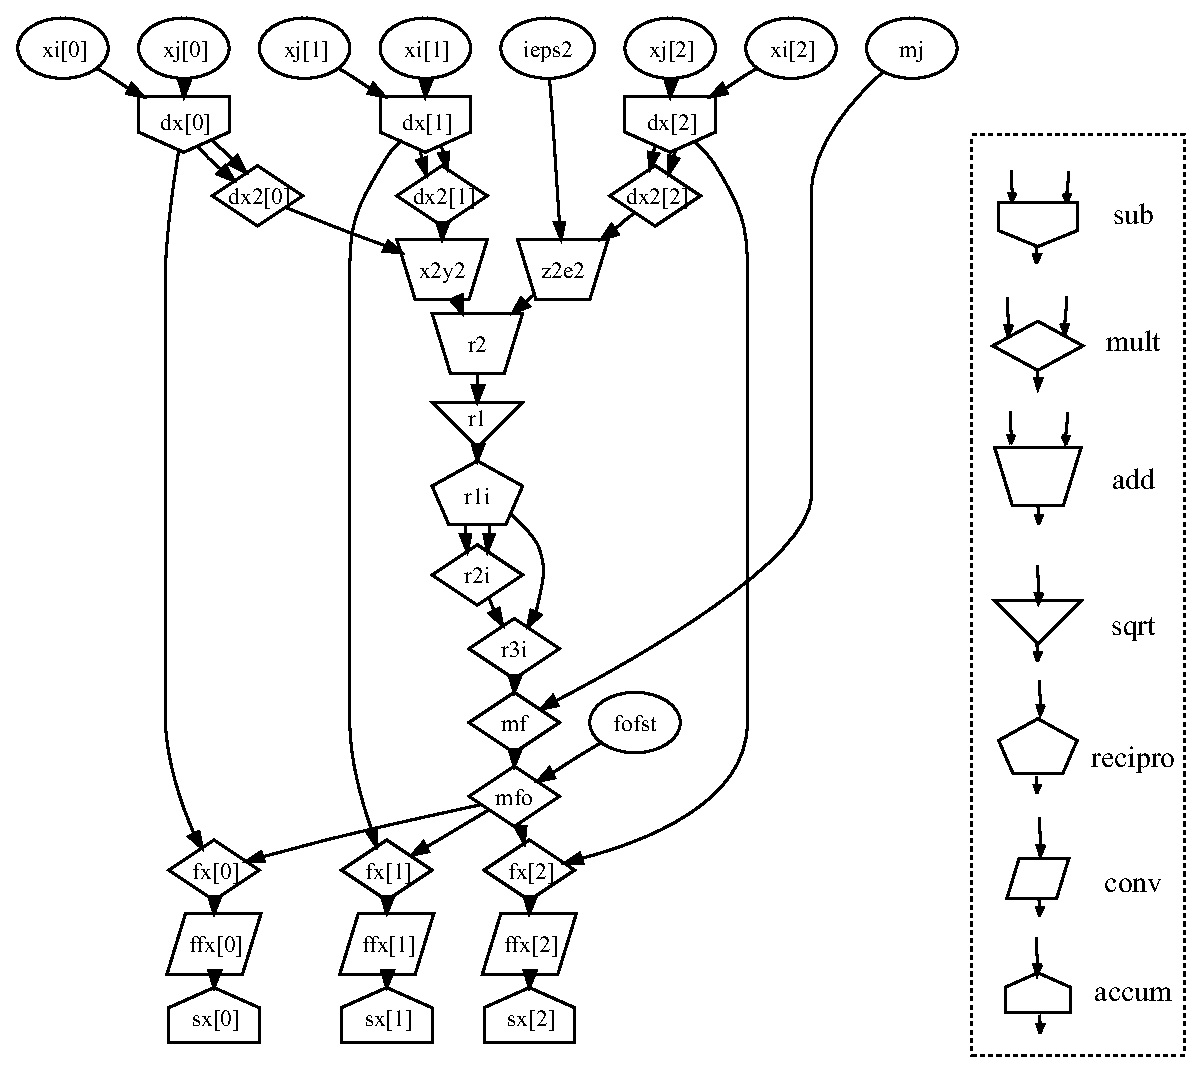
\includegraphics[angle=+0,width=8cm]{./mat/grav_float_nodelay.eps}
\caption{Simple data flow of gravitational force pipeline.}
\label{fig_grav_float_nodelay}
\end{center}
\end{figure}

\begin{figure}[htb]
\begin{center}
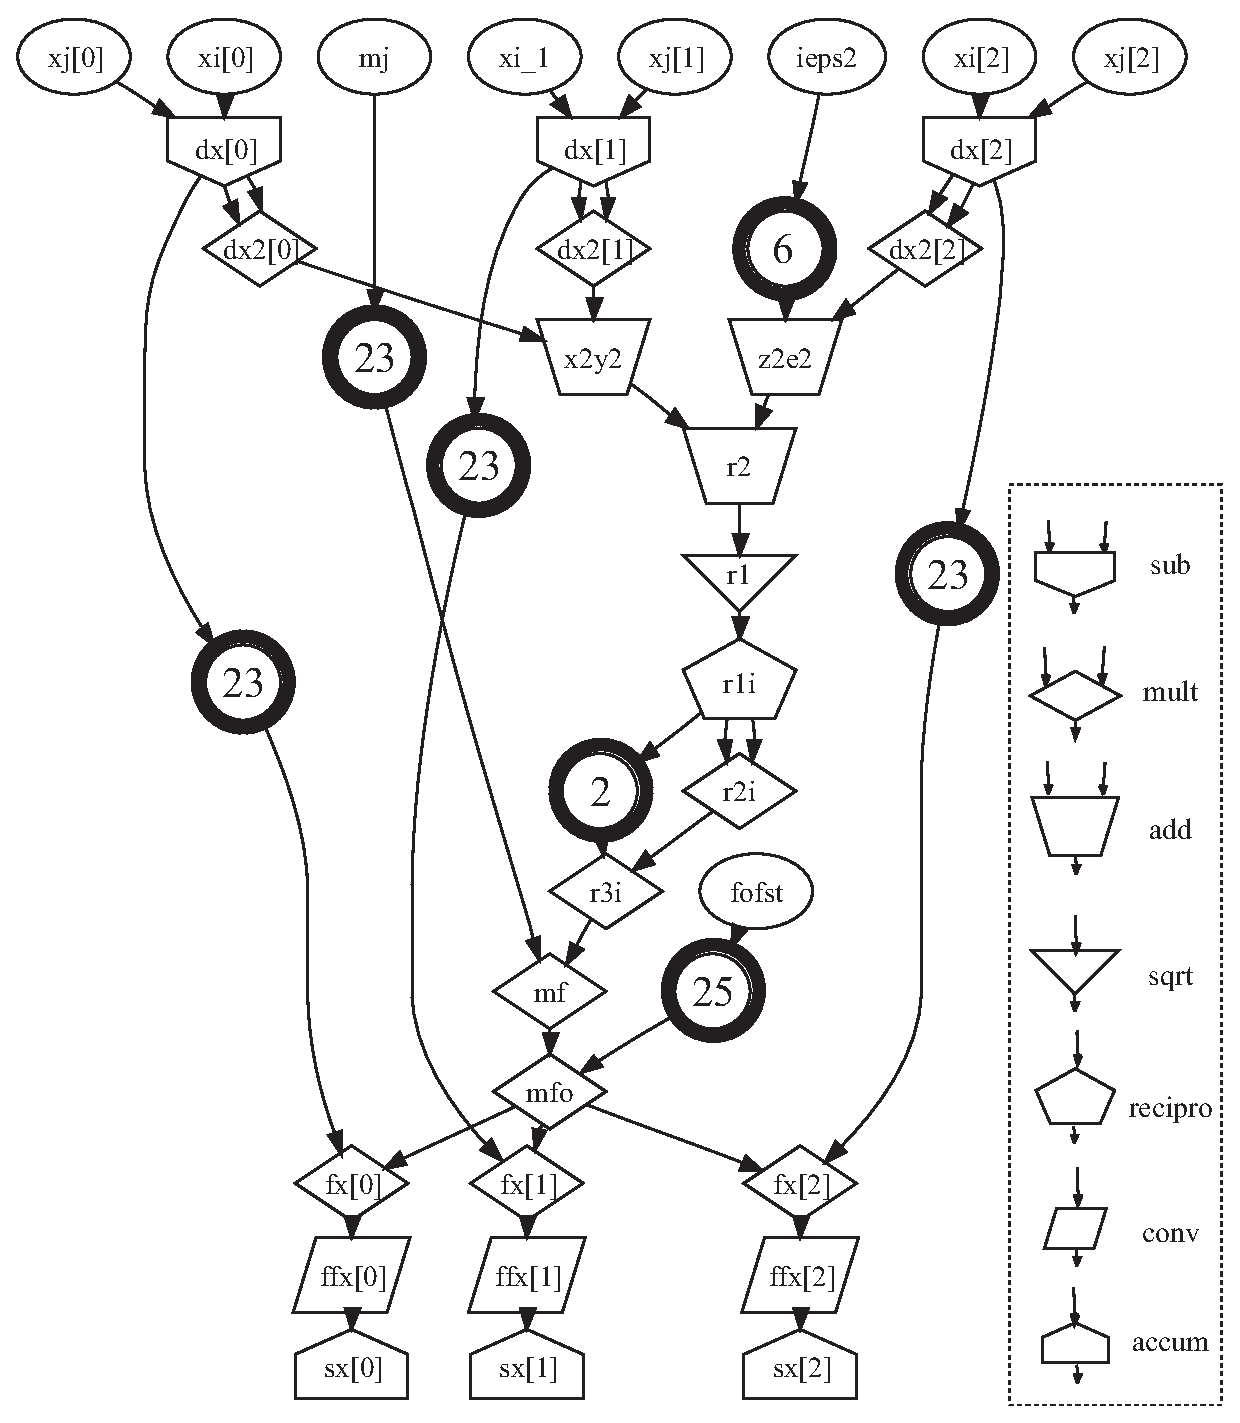
\includegraphics[angle=+0,width=8cm]{./mat/grav_float_delay.eps}
\caption{Delay inserted data flow of gravitational force pipeline.}
\label{fig_grav_float_delay}
\end{center}
\end{figure}


\begin{table*}
\caption{Implementation result and comparison with other implementation}
\begin{center}
\begin{tabular}{lccc}
\hline
\hline
                     & GRAPE-5 board(8 ASICs) & \multicolumn{2}{c}{PROGRAPE-3 board(4 FPGAs)}  \\
\hline
format :input        & 32-bit fixed point  & 26-bit floating point & 32-bit fixed point \\
format :internal     & 17-bit logarithmic  & 26-bit floating point & 17-bit logarithmic \\
format :accumulation & 64-bit fixed point  & 64-bit fixed point    & 64-bit fixed point \\
A number of PEs      & 16                  &   24                  &   64               \\
perk performance(Gflops)    & 48.6         & 60.8                  & 162.1              \\
pair-wise error             & 10$^{-2.4}$   &  10$^{-4.8}$ & 10$^{-2.4}$                \\

\hline
\hline
\end{tabular}
\end{center}
\label{tabcompg5}
\end{table*}

\begin{figure}[htb]
\begin{center}
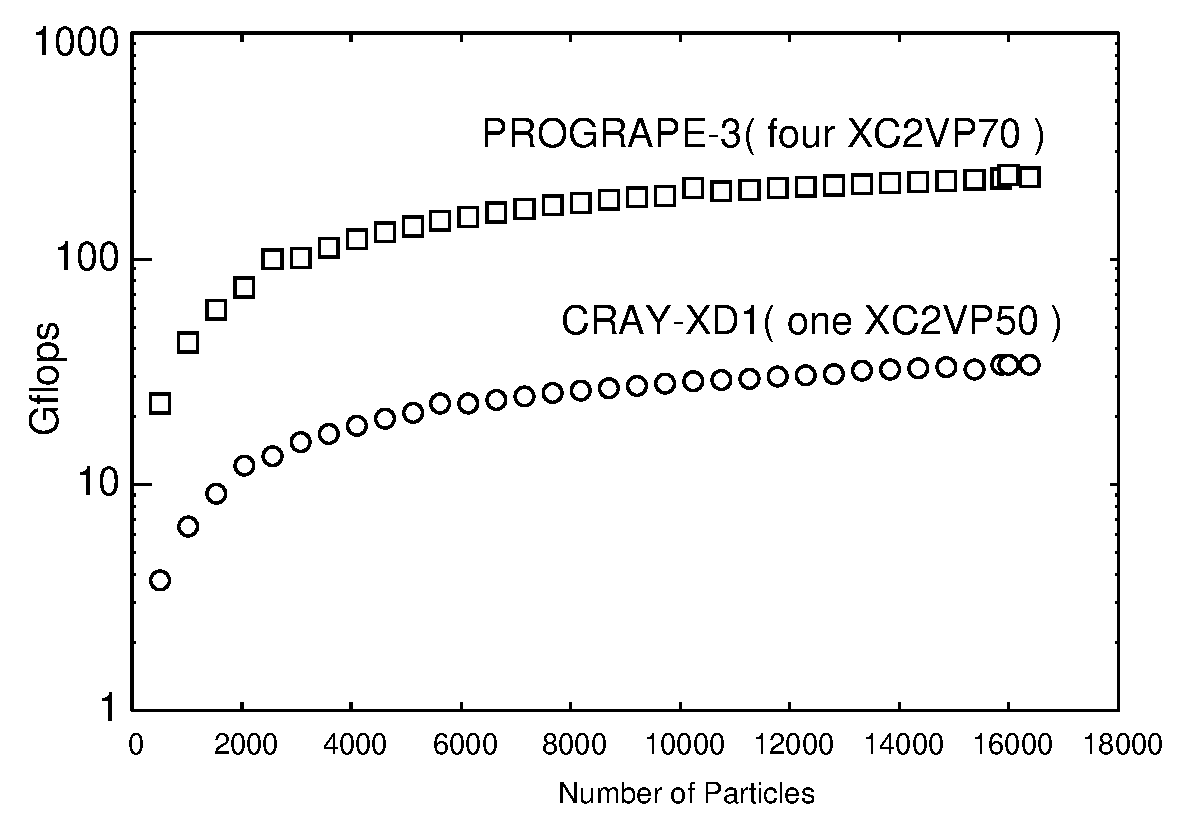
\includegraphics[angle=+0,width=8cm]{./mat/perform/graph.eps}
\caption{The mesured caluclation speed of single PROGRAPE-3 board in Gflops for the direct-summation algorithm, plotted as functions of the number of particles, N.}
\label{MESURE-PERFORM}
\end{center}
\end{figure}


\section{Related work}
\section{Larated work}
%%PROGRAPE-1
An earlier example of the use of reconfigurable hardware in the
acceleration of scientific computations is PROGRAPE-1(PROgrammable
GRAPE-1)\ref{Hamada2000}. PROGRAPE-1 is an FBA for many-body
simulations. It is implemented with two Altera EPF10K100 FPGAs, each
of which contains about 100k gates. The peak performance of
calculating gravitational force results in 0.96 Gflops.  PROGRAPE-1
was composed of short length(14-bit) logarithmic arithmetics and this
was the reason why the performance was excelent with this outdated
FPGAs.

%%RACE
MPRACE\footnote{\tt http://www-li5.ti.uni-mannheim.de/fpga/race/} is
similar system to PROGRAPE-1, which uses a parameterized
floating-point library\cite{GKM02}.  The target application of MPRACE
is astrophysical hydrodynamics simulations using SPH(Smoothed Particle
Hydrodynamics) method.  They are making an effort to construct a high
performance system.


%%CAST
CAST(Computer Arithmetic Synthesis Tool)\ref{THYL04} is a similar tool
to our PGR.  The contribution of both tools is a set of parametrized
floating-point, fixed-point, and logarithmic numbers libraries and a
tool that generates a computational pipeline from an abstract description.
The CAST developers claimed that they have implemented
a pipeline for gravitational N-body problem. 
However, they have only indicated 
projected results based on simulation with only one pipeline unit.
There is a big distance between implementing a pipeline unit and building a real
high-performance commutating system. In contrast to their work,
we have implemented 64 pipelines (16 pipelines per one FPGA chip)
for gravitational N-body problem on our target hardware PROGRAPE3 board,
and the mesured highest performance of our system
(Opteron 2.4GHz PC + one PROGRAPE-3 board) is 100 GFLOPS as shown in Figure \ref{MESURE-PERFORM}.
We have proved a real high-performance computing system
can be implemented using the PGR.

%%MARGE

\section{Conclusion}
We have developed the PGR package, a software which automatically generate
most of communication softwares and the hardware descriptions
(the bit-level hardware design of pipeline processors)
for FBAs from a high-level description PGDL.
Using the PGR package, we have implemented gravitational force
pipelines used in astrophysical simulations.
The PGDL description for the gravitational force pipelines
is only a several tens of lines of a text file.
Regardless of a very simple description, we could obtain very
efficient implementation. 
Using PGR, we will reach the design area where nobody can achieve.

%------------------------------------------------------------------------- 
\bibliographystyle{latex8}
\begin{thebibliography}{}

\bibitem{Splash}
Buell, D., A., Arnold, J., M., Kleinfelder, W. J.:
Splash 2: FPGAs in a custom computing machine.
IEEE Computer Society Press, Los Alamitos.
(1996)

\bibitem{Hamada2000}
Hamada,~T., Fukushige,~T., Kawai,~A., \& Makino,~J.:
PROGRAPE-1: A Programmable, Multi-Purpose Computer for Many-Body Simulations.
Publication of Astronomical Society of Japan.
{\bfseries 52} (2000) 943--954

\bibitem{KFMT00}
Kawai,~A., Fukushige,~T., Makino,~J., \& Taiji,~M.:
GRAPE-5: A Special-Purpose Computer for N-body Simulation.
Publication of Astronomical Society of Japan.
{\bfseries 52} (2000) 659--676

\bibitem{Makino1990}
Makino, J., Ito, T., \& Ebisuzaki, T.:
Error Analysis of the GRAPE-1 Special-Purpose N-Body Machine.
Publication of Astronomical Society of Japan.
{\bfseries 42} (1990) 717--736

\bibitem{GRAPE}
Makino,~J., \& Taiji,~M.:
Scientific Simulations with Special-Purpose Computers --- The GRAPE Systems.
Chichester: John Wiley and Sons.
(1998)

\bibitem{GKM02}
Lienhart, G, L., Kugel, A., \& M{\"a}nner, R.:
Using Floating Point Arithmetic on FPGAs to Accelerate Scientific N-Body Simulations.
Proc. of IEEE FCCM'02 Symposium on Field-Programmable Custom Computing Machines, 
Los Alamitos, CA.
(2002) 182--191

\bibitem{DP}
Sankoff, D., \& Kruska, J.:
Time Warps, String Edits, and Macromeleclues:
The Theory and Practice of Sequence Comparison, (Reading: Addison-Wesley).
(1983)

\bibitem{THYL04}
Tsoi, K., Ho, C., Yeung, H., \& Leong, P.:
An Arithmetic Library and its Application to the N-body Problem.
Proc. of IEEE Symposium on Field-Programmable Custom Computing Machines, 
IEEE Computer Society Press.
(2004) 68--78

\bibitem{W93}
Wazlowski, M., Agarwal, L., Lee, T., Smith, A., Lam, E., Athanas, P., Silverman, H. \& Ghosh, S.:
PRISM-II compiler and architecture. 
Proc. of IEEE FCCM'93 Symposium on Field-Programmable Custom Computing Machines, 
Los Alamitos, CA.
(1993) 9--16 

\bibitem{VBRSTB94}
Vuillemin, J., Bertin, P., Roncin, D., Shand, M., Touati, H., \& Boucard, P.:
Programmable active memories: Reconfigurable systems come of age.
IEEE Transactions on VLSI Systems.
(1996) 56--69

\end{thebibliography}

\end{document}
